% !TeX spellcheck = en_US
%\documentclass[11pt,a4paper]{article}
\documentclass[11pt
  , a4paper
  , article
  , oneside
%  , twoside
%  , draft
]{memoir}

\usepackage{control}
\usepackage{kotex}
\usepackage[numbers]{natbib}
%\usepackage[pdftex]{graphicx}
%\DeclareGraphicsExtensions{.pdf,.png,.jpg}
\begin{document}

\newcommand{\technumber}{
  Digital Signal Processing using MATLAB}
\title{\textbf{Digital Signal Processing: 실습 11 \\
		제5장 이산 푸리에 변환 \\}}

\author{이상일\thanks{silee7103@ibs.re.kr} \\

  학번: 201460437\\
  Computer Engineering, Chungnam National University 
}
\date{\today}

\renewcommand{\maketitlehooka}{\begin{flushright}\textsf{\technumber}\end{flushright}}
%\renewcommand{\maketitlehookb}{\centering\textsf{\subtitle}}
%\renewcommand{\maketitlehookc}{C}
%\renewcommand{\maketitlehookd}{D}

\maketitle

\begin{abstract}
MATLAB을 사용한 Digital Signal Processing에 대한 실습과제에 대한 Documents를 구성한다.
\end{abstract}


\chapter{Example 5-15:}

\begin{lstlisting}[style=termstyle]
% Example 05.15

%a:
x1 = [1,2,2]; x2 = [1,2,3,4]; 
y = circonvt(x1,x2,5)

%b:
x1 = [1,2,2]; x2 = [1,2,3,4]; y = circonvt(x1,x2,6)
\end{lstlisting}

\begin{figure}[h!]
	\centering
	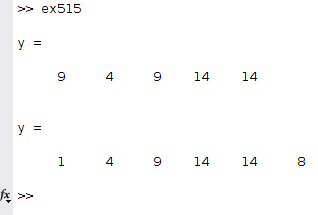
\includegraphics[width=0.4\textwidth,height=0.2\textwidth]{./images/ex515.png}
	\caption{Example 5.15 Result}
	\label{fig:Example 5.15 Result}
\end{figure}

\chapter{Example 5-16:}
\begin{lstlisting}[style=termstyle]
% Example 05.16

%a:
x1 = [1,2,2,1]; x2 = [1,-1,-1,1]; x3=conv(x1,x2)

%b:
x4 = circonvt(x1,x2,7)
\end{lstlisting}

\begin{figure}[h!]
	\centering
	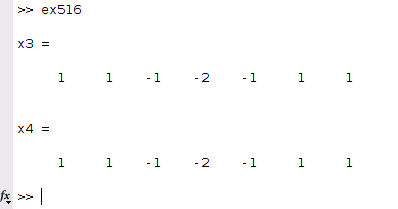
\includegraphics[width=0.4\textwidth,height=0.2\textwidth]{./images/ex516.png}
	\caption{Example 5.16 Result}
	\label{fig:Example 5.61 Result}
\end{figure}

\chapter{Example 5-17:}
\begin{lstlisting}[style=termstyle]
 Example 5.17
 
 x1 = [1,2,2,1]; x2 = [1,-1,-1,1]; x3=conv(x1,x2)
 
 % N = 6:
 x4 = circonvt(x1,x2,6)
 %Error
 err_6 = x4-x3(1:6)
 
 % N = 5:
 x4 = circonvt(x1,x2,5)
 %Error
 err_5 = x4-x3(1:5)
 
 % N = 4:
 x4 = circonvt(x1,x2,4)
 %Error
 err_4 = x4-x3(1:4)
\end{lstlisting}

\begin{figure}[h!]
	\centering
	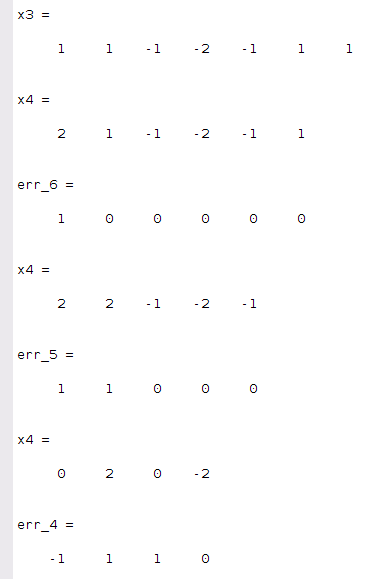
\includegraphics[width=0.5\textwidth,height=0.4\textwidth]{./images/ex517.png}
	\caption{Example 5.17 Result}
	\label{fig:Example 5.17 Result}
\end{figure}

\clearpage

\chapter{Example 5-19:}
\begin{lstlisting}[style=termstyle]
 Example 5.19
 
 n = 0:9; x = n+1; h = [1,0,-1]; N = 6; y = ovrlpsav(x,h,N)
\end{lstlisting}

\begin{figure}[h!]
	\centering
	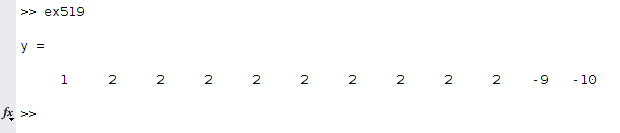
\includegraphics[width=0.4\textwidth,height=0.2\textwidth]{./images/ex519.png}
	\caption{Example 5.19 Result}
	\label{fig:Example 5.19 Result}
\end{figure}

\chapter{Example 5-22:}
\begin{lstlisting}[style=termstyle]
% Example 5.22

Nmax = 2048; fft_time=zeros(1,Nmax);

for n=1:1:Nmax
%disp(n);
%x=ones(1,n);
x=rand(1,n);
t=clock;fft(x);fft_time(n)=etime(clock,t);
end

n=[1:1:Nmax];
plot(n,fft_time,'.');

axis([0,2500,0,50])
xlabel('N');ylabel('Time in Sec.')
title('FFT execution times')
\end{lstlisting}

본 예제는 MATLAB 2014a 버전에서는 아래 그림에서와 같이 확인이 불가능 하였다.

\begin{figure}[h!]
	\centering
	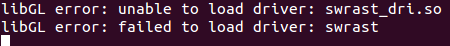
\includegraphics[width=0.3\textwidth,height=0.06\textwidth]{./images/ex522.png}
	\caption{Example 5.22 Result}
	\label{fig:Example 5.22 Result}
\end{figure}

\subsection{Example 5-23}
\begin{lstlisting}[style=termstyle]
% Example 5.23
conv_time = zeros(1,150); fft_time = zeros(1,150);
for N = 1:150
tc = 0; tf=0;
L = 2*N-1; nu = round((log10(L)/log10(2))+0.45); L = 2^nu;
for I=1:100
h = randn(1,N);
x = rand(1,N);
t0 = clock; y1 = conv(h,x); t1=etime(clock,t0);
tc = tc+t1;
t0 = clock; y2 = ifft(fft(h,L).*fft(x,L)); t2=etime(clock,t0);
tf = tf+t2;
end
conv_time(N)=tc/100;
fft_time(N)=tf/100;
end

n = 1:150; subplot(1,1,1);
plot(n(25:150),conv_time(25:150),n(25:150),fft_time(25:150))
save times.txt conv_time fft_time -ascii -tabs
\end{lstlisting}

\begin{figure}[h!]
	\centering
	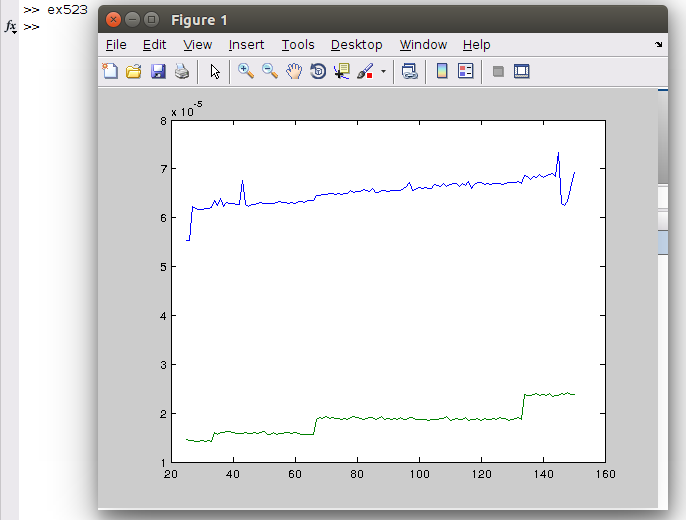
\includegraphics[width=0.5\textwidth,height=0.4\textwidth]{./images/ex523.png}
	\caption{Example 5.23 Result}
	\label{fig:Example 5.23 Result}
\end{figure}


\chapter{Example 5.6.6}
High-speed Block Convolution 구현은 아래와 같다.

\begin{lstlisting}[style=termstyle]
function [y] =  hsolpsav(x,h,N)
% High-speed Overlap-Save method of block convolutions using FFT
% --------------------------------------------------------------
% [y] = hsolpsav(x,h,N)
% y = output sequence
% x = input sequence
% h = impulse response
% N = block length (must be a power of two)

N = 2^(ceil(log10(N)/log10(2));
Lenx = length(x); M = length(h);
M1 = M-1; L = N-M1;
h = fft(h,N);
x = [zeros(1,M1), x, zeros(1,N-1)];
K = floor((Lenx+M1-1)/(L)); % # of blocks
Y = zeros(K+1,N);
for k=0:K
xk = fft(x(k*L+1:k*L+N));
Y(k+1,:) = real(ifft(xk.*h));
end
Y = Y(:,M:N)'; y = (Y(:))';
\end{lstlisting}

\chapter{Common: M-Functions}
circonvt.m:
\begin{lstlisting}[style=termstyle]
function y = circonvt(x1,x2,N)
% N-point circular convolution between x1 and x2: (time-domain)
% -------------------------------------------------------------
% [y] = circonvt(x1,x2,N)
%  y = output sequence containing the circular convolution
% x1 = input sequence of length N1 <= N
% x2 = input sequence of length N2 <= N
%  N = size of circular buffer
%  Method: y(n) = sum (x1(m)*x2((n-m) mod N))

% Check for length of x1
if length(x1) > N
error('N must be >= the length of x1')
end

% Check for length of x2
if length(x2) > N
error('N must be >= the length of x2')
end

x1=[x1 zeros(1,N-length(x1))];
x2=[x2 zeros(1,N-length(x2))];

m = [0:1:N-1];

x2 = x2(mod(-m,N)+1);
H = zeros(N,N);

for n = 1:1:N
H(n,:) = cirshftt(x2,n-1,N);
end
\end{lstlisting}

ovrlpsav.m:
\begin{lstlisting}[style=termstyle]
ffunction [y] = ovrlpsav(x,h,N)
% Overlap-Save method of block convolution
% ----------------------------------------
% [y] = ovrlpsav(x,h,N)
% y = output sequence
% x = input sequence
% h = impulse response
% N = block length
%
Lenx = length(x); M = length(h);
M1 = M-1; L = N-M1;
h = [h zeros(1,N-M)];
x = [zeros(1,M1), x, zeros(1,N-1)]; % preappend (M-1) zeros
K = floor((Lenx+M1-1)/(L));         % # of blocks
Y = zeros(K+1,N);
% convolution with succesive blocks
for k=0:K
xk = x(k*L+1:k*L+N);
Y(k+1,:) = circonvt(xk,h,N);
end
Y = Y(:,M:N)';                      % discard the first (M-1) samples
y = (Y(:))';                        % assemble output

\end{lstlisting}

\end{document}

